\chapter{Global Project Organization}
\label{vl:tc-global}

\section{Global Project Partners}
\label{sec:partners}

The \dword{lbnf} project is responsible for providing both the
\dword{cf} and supporting infrastructure (cryostats and
cryogenics systems) that house the \dword{dune} \dword{fd}
modules. \dword{lbnf} is a USA \dword{doe} project incorporating
contributions from international partners and is headed by the
\dword{lbnf} project director who also serves as the \dword{fnal}
deputy director for \dword{lbnf}.  
\fixme{we've been doing titles lower case... anne}
The international \dword{dune}
collaboration under the direction of its management team is
responsible for the detector components.  The \dword{dune} \dword{fd}
construction project encompasses all activities required for designing
and fabricating the detector elements and incorporates contributions
from a number of international partners.  The organization of the
global \dword{lbnf-dune}, which encompasses both project elements, is
shown in Figure~\ref{fig:DUNE_global}.
\begin{dunefigure}[Global project organization]{fig:DUNE_global}
  {\dword{lbnf-dune} organization.}
  \includegraphics[width=0.95\textwidth]{FS_Integration_OrgChart_notitle}
\end{dunefigure}

In addition to the \dword{lbnf} and \dword{dune} pieces, the overall
coordination of installation activities in the underground caverns 
is managed as a separate element of \dword{lbnf-dune} under the
responsibility of the \dword{ipd}, who is appointed by and reports
to the \dword{fnal} director.  To ensure coordination across
all elements of \dword{lbnf-dune}, the \dword{ipd} connects to both
the facilities and detector construction projects through ex-officio
positions on the \dword{lbnf} Project Management Board and
\dword{dune} \dword{exb}, respectively.  In carrying out these
responsibilities, the \dword{ipd} receives support from the \dword{sdsd},
a \dword{fnal} division established to 
provide the necessary supporting infrastructure for installation, commissioning, and operation 
of the \dword{dune} detector.
 \fixme{I moved up the definition of SDSD from the end of the chapter. anne}
%The head of the \dword{sdsd} works closely with \dword{surf}.
% to ensure that appropriate site infrastructure and support mechanisms 
%needed to execute onsite project activities are in place.

The \dword{ipd} works closely with the \dword{lbnf} and \dword{dune}
teams in advance of these activities to coordinate planning
and ensure that detector elements are properly integrated within the 
supporting infrastructure.  Although the \dword{ipd} is responsible 
for overall coordination of  installation activities
at \dword{surf}, the \dword{dune} consortia maintain responsibility 
for the installation and commissioning of their detector subsystems
and support these activities by providing dedicated personnel and
equipment resources.  Likewise, \dword{lbnf} retains responsibility
for the installation and commissioning of supporting infrastructure
items and provides dedicated resources to support these activities.          

\section{Experimental Facilities Interface Group}
\label{sec:efig}

The \dword{efig} is the body responsible for the required high-level
coordination between the \dword{lbnf} and \dword{dune} construction 
projects.  The \dword{lbnf} project director and \dword{ipd} 
co-chair the \dword{efig}.  \dword{efig} leadership also incorporates 
the four members of the \dword{dune} collaboration management 
team (co-spokespersons, \dword{tcoord}, and \dword{rcoord}).  
The \dword{efig} is responsible for steering the integration and   
installation of the \dword{lbnf-dune} pieces and operates via the 
consensus of its leadership team.  If issues arise for which consensus 
cannot be achieved, decision-making responsibility is passed to the 
\dword{fnal} Director.

\section{Joint Project Office}
\label{sec:jpo}

The \dword{efig} is augmented by a \dword{jpo} that supports both 
the \dword{lbnf} and \dword{dune} projects as well as the integration
effort that connects the two together. The \dword{jpo} combines
project support functions that exist within the different elements 
of global project to ensure proper coordination across the entire 
\dword{lbnf-dune} enterprise.  Project functions coordinated globally 
through the \dword{jpo} are shown in Figure~\ref{fig:DUNE_jpo} along 
with the personnel currently supporting those functions.  The team 
members who support these functions within the \dword{jpo} framework
are drawn from the \dword{lbnf} project office, \dword{dune} \dword{tc}, 
and \dword{lbnf}/\dword{dune} \dword{integoff} personnel.  
\begin{dunefigure}[JPO functions]{fig:DUNE_jpo}
  {\dword{jpo} global support functions and teams}
  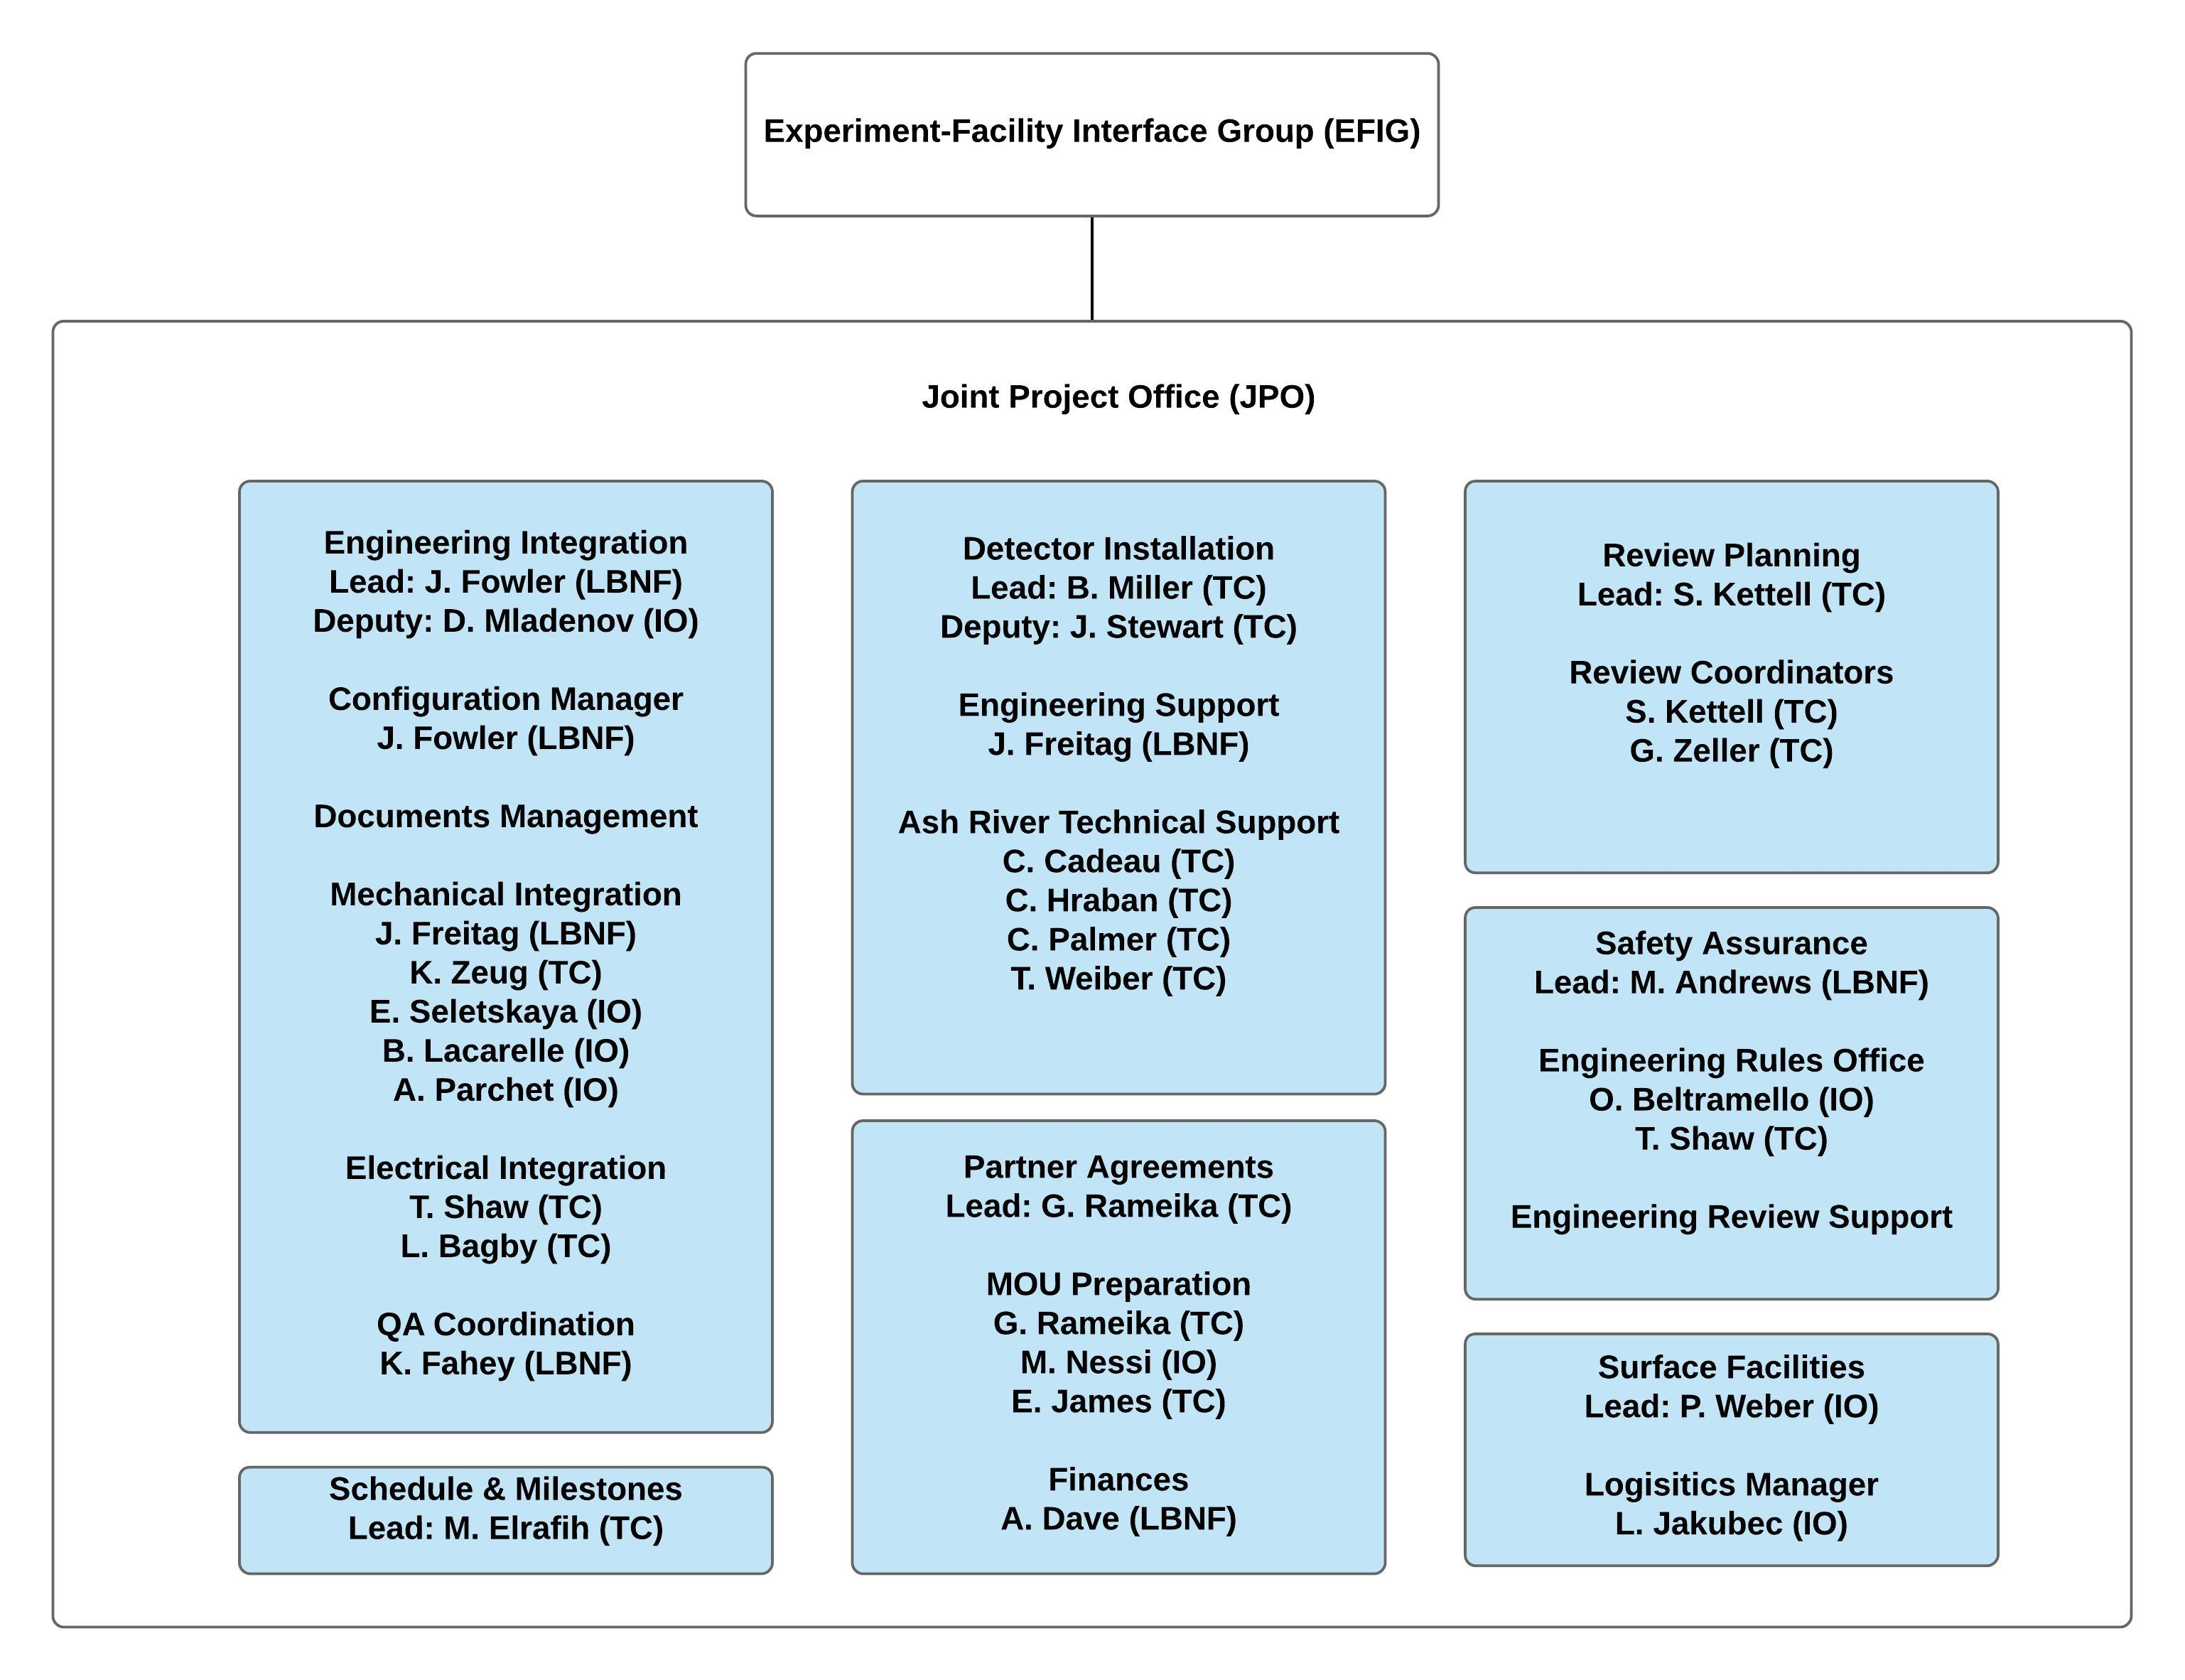
\includegraphics[width=0.85\textwidth]{JPO_OrgChart_v4}
\end{dunefigure}
Team members focusing on specific project activities and functions 
within the \dword{jpo} are typically those carrying equivalent 
responsibilities within their home organization.  For example, 
the \dword{jpo} team responsible for building the fully integrated 
\threed CAD model of the detector within its supporting infrastructure 
and surrounding facility includes the members of the \dword{lbnf} and 
\dword{dune} project teams responsible for integrating the individual 
elements.

\section{Coordinated Global Project Functions}
\label{sec:global_project}

Project support functions requiring \dword{jpo} coordination include
safety, engineering integration, change control and document 
management, scheduling, review planning and oversight, and development 
of partner agreements.  Additional detail is provided in the subsequent 
sections regarding the \dword{jpo} role in coordinating these support 
functions.

Planning activities related to detector installation and the provision 
of surface facilities are also currently embedded within the framework 
of the \dword{jpo} to ensure that all project elements are properly 
incorporated.  At the time when \dword{lbnf} \dword{fscf} delivers 
\dword{aup} of the underground detector caverns at \dword{surf}, the 
coordination of onsite activities associated with detector installation 
and the operation of surface facilities will be fully embedded within 
the \dword{lbnf}/\dword{dune} \dword{integoff} under the direction of the \dword{ipd}.  
Some current members of the \dword{lbnf} project office and \dword{dune}
\dword{tc} are expected to be moved into the \dword{integoff} at that point in time.  
The \dword{integoff} team required to coordinate post-excavation activities at 
\dword{surf} is described in Chapter~\ref{ch:tc-jpo}.  

\subsection{Safety}
\label{sec:dune_safety}

To ensure a consistent approach to safety across \dword{lbnf-dune},
there is a single \dword{lbnf-dune} \dword{esh} manager who reports 
to the \dword{lbnf} project director, \dword{ipd}, and \dword{dune}
management (via the \dword{dune} \dword{tcoord}).  This individual
directs separate safety teams responsible for implementing the
\dword{lbnf-dune} \dword{esh} program within both the \dword{lbnf} 
and \dword{dune} projects as well as the \dword{lbnf}/\dword{dune}
installation activities at \dword{surf}. The safety organization 
is shown in Figure~\ref{fig:dune_esh} and is described further in
Sections~\ref{sec:tc_safety} and~\ref{sec:far_site_safety}, and in 
Chapter~\ref{vl:tc-ESH}.
\begin{dunefigure}[\dshort{lbnf-dune} \dshort{esh}]{fig:dune_esh}
  {High level \dword{lbnf-dune} \dword{esh} organization.}
  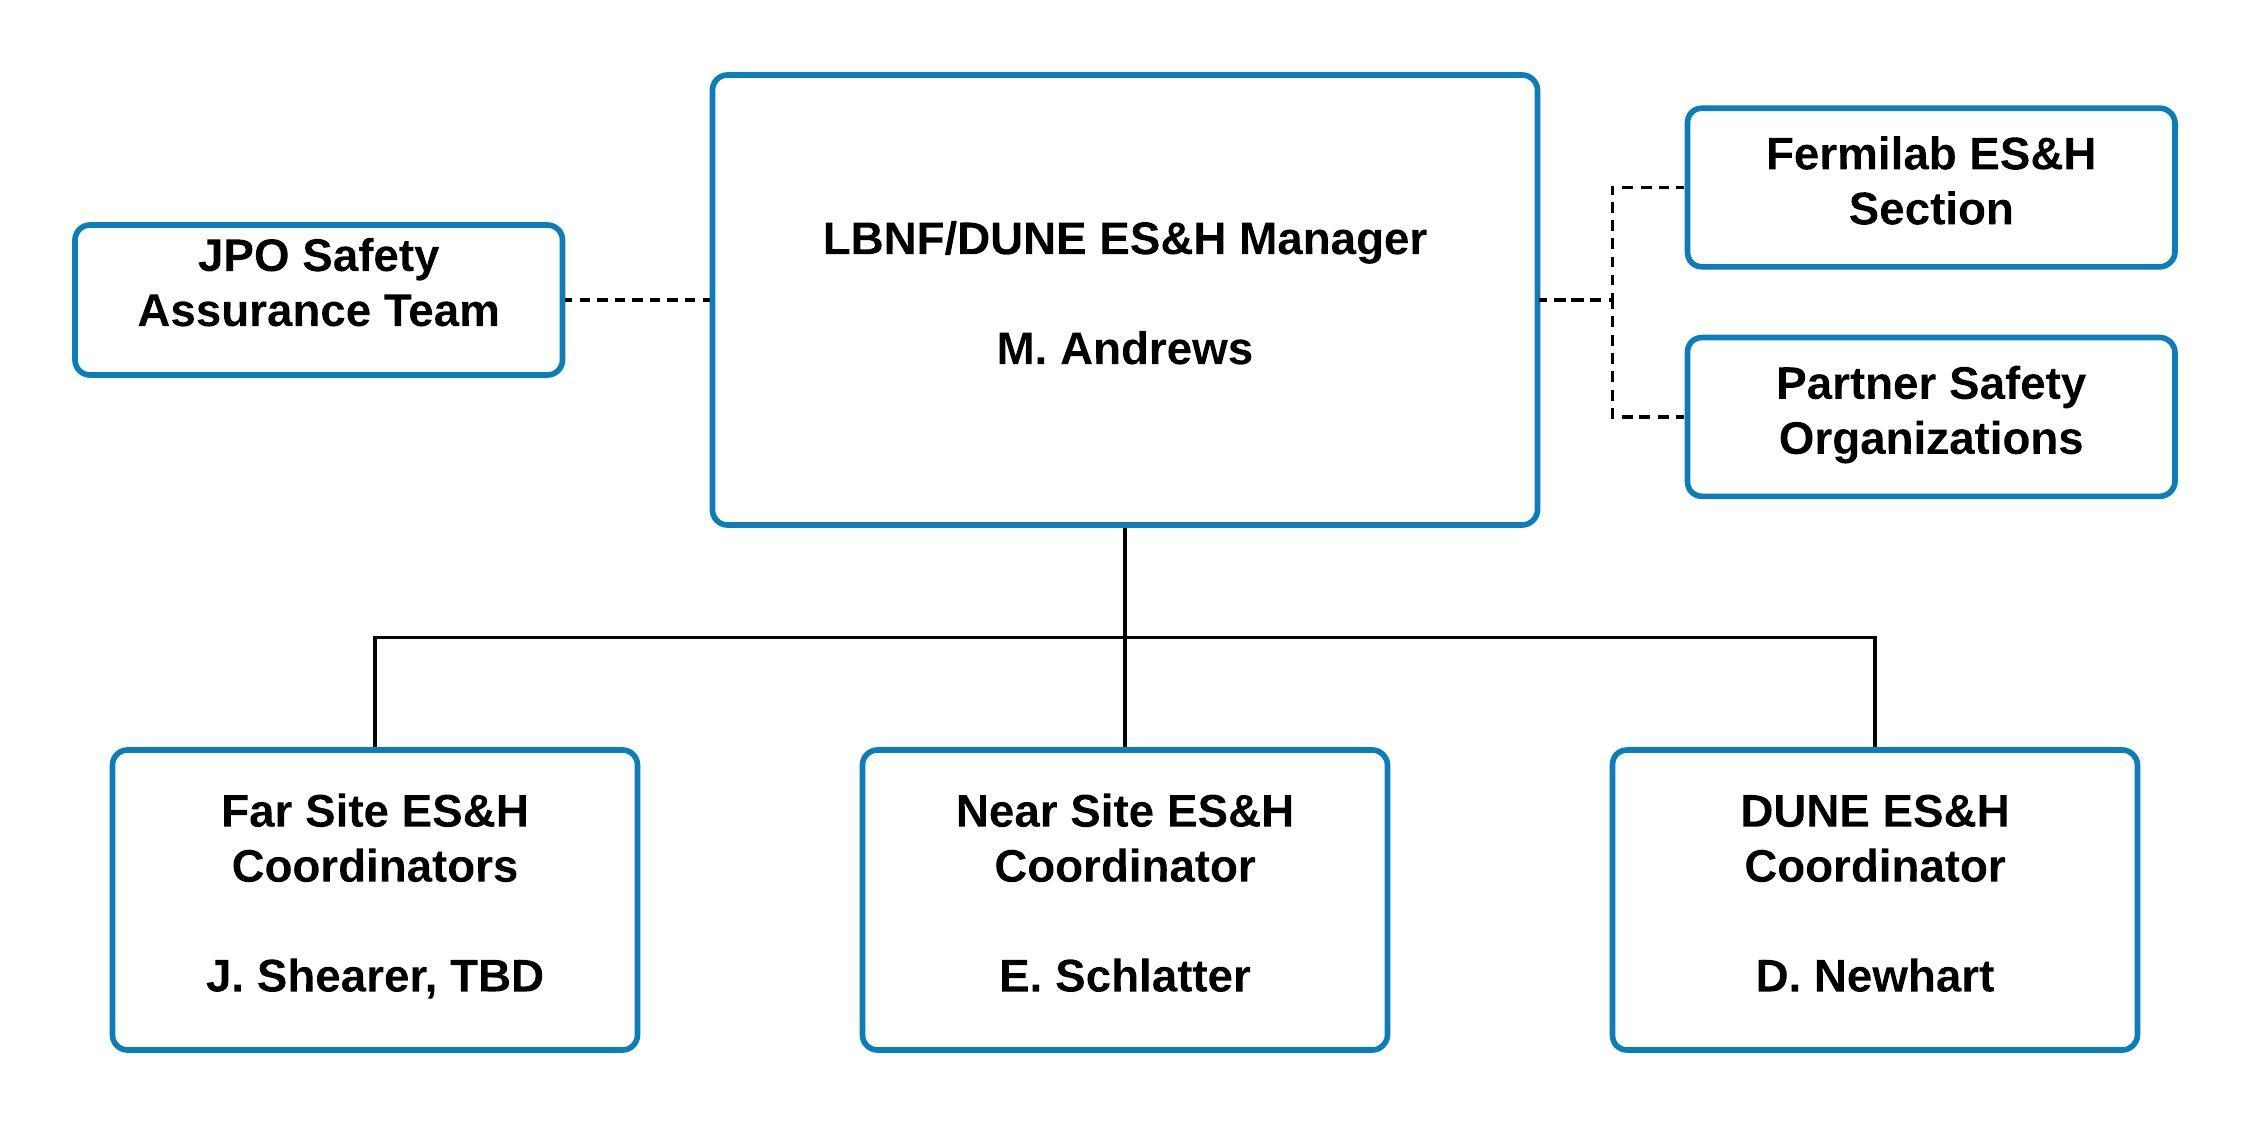
\includegraphics[width=0.85\textwidth]{DUNE_Safety_Org_Chart_v2}
\end{dunefigure}
The \dword{lbnf-dune} \dword{esh} manager works with the \dword{fnal} 
and \dword{surf} safety organizations to ensure that all project-related 
activities comply with the rules and regulations of the host 
organizations.  For example, the \dword{lbnf-dune} \dword{esh} manager 
works with the host safety organizations to develop the rules and 
regulations governing work in the underground areas at \dword{surf}, 
which are then consistently applied across all underground project 
activities.

The \dword{jpo} engineering safety assurance team defines a common 
set of design and construction rules (mechanical and electrical) to 
ensure consistent application of engineering standards and engineering 
documentation requirements across \dword{lbnf-dune}.  This team works 
with the \dword{lbnf-dune} \dword{esh} manager to develop equivalencies 
in codes and standards across the international project as needed.  
Following on lessons-learned from the processes employed for the 
\dword{protodune} detectors, an important mandate of the engineering 
safety assurance team is to ensure that safety issues related to 
component handling and installation are incorporated within the 
earliest stages of the design review process.  The \dword{jpo} team 
incorporates engineering resources to perform independent validation 
of required mechanical analyses that ensure the structural integrity 
of detector components through all stages of construction, installation, 
and operation.

\subsection{Engineering Integration}
\label{sec:dune_engineering}

A central \dword{jpo} engineering team is responsible for building 
an integrated model of the detectors within their supporting
infrastructure and the \dword{fscf} that house them.  The team
builds and maintains a full \threed CAD model of everything in the
underground detector caverns from the models of the individual
components provided by the \dword{lbnf} and \dword{dune} design 
teams.  Starting from the latest, approved version of the full CAD 
model, the \dword{jpo} team incorporates approved changes as they 
are received and checks to ensure that no errors or spatial conflicts 
are introduced into the model.  As part of this process \twod control 
drawings are produced from the \threed CAD model to validate adherence 
with critical component-to-component clearances within the integrated
model.  The updated working model is passed back to the individual
\dword{lbnf} and \dword{dune} design teams to validate that their
design modifications have been properly incorporated within the 
global model.  After receiving the appropriate sign-offs from all 
parties, the \dword{jpo} team tags a new frozen release of the model 
and makes it available to the design teams as the current release 
against which the next set of design changes will be generated.

Electrical engineers are incorporated within the central \dword{jpo} 
team to ensure proper integration of the detector electrical 
components.  This team is responsible for ensuring that detector 
grounding and shielding requirements, the maintenance of which are 
critical for detector performance, are strictly adhered to.  The 
team oversees the layout of electronics racks and cable trays both 
on the top of the cryostats and within the \dword{cuc} counting room 
that hosts the \dword{daq} electronics.  It also oversees the design 
of the power and cooling distribution systems that are required to 
support the electronics infrastructure.

The \dword{jpo} engineering team is responsible for documenting and
controlling the interfaces between the \dword{lbnf} and \dword{dune} 
projects as well as the interfaces between these projects and the 
\dword{lbnf}/\dword{dune}  installation activities at \dword{surf}.  
To define these interfaces, the \dword{jpo} team develops formal 
documents which, subsequent to the approval of the relevant managers, 
are placed under signature and versioning control.  These documents 
are monitored regularly to ensure that no missing scope or technical 
incompatibilities are introduced at the boundaries between the projects.

\subsection{Change Control and Document Management}
\label{sec:dune_changecontrol}

The \dword{lbnf-dune} project partners have agreed to adopt 
the formal change control process developed previously for the 
\dword{lbnf} project.  The change control process applies to 
proposed modifications of requirements, technical designs, 
schedule, overall project scope and assigned responsibilities 
for individual scope items.  The formal \dword{lbnf-dune} 
change control process is described in~\citedocdb{82}.  The 
process includes separate decision paths for items affecting 
only \dword{dune} or \dword{lbnf} and incorporates an additional 
pathway for items affecting both projects.  A hierarchy of 
decision-making layers is built into each pathway based on 
pre-determined thresholds related to the extent of the proposed 
change.  The lowest-level change control body for modifications 
affecting both \dword{lbnf} and \dword{dune} is the \dword{efig}.  
The \dword{jpo} incorporates a configuration manager within the 
engineering integration team who is responsible for formally 
implementing changes that are approved through this process.  
After technical changes are incorporated into the global \threed 
CAD models, the engineering integration team is responsible for 
checking production drawings and verifying that no potential 
space conflicts have been introduced.  Under the direction of 
the configuration manager, all project changes are documented 
in detail and approved by the appropriate project partners using 
the \dword{lbnf} change control tool.

The configuration manager oversees a document management team
responsible for %administrating 
administering and managing the \dword{lbnf-dune}
%document management system, which is hosted in the \dword{edms}.  
%All technical documents and drawings are stored in the \dword{edms} system
%under formal signature and versioning control.  A product breakdown
document management system used for all technical documents 
and drawings. This system, \dword{edms}, stores these documents and maintaines them  
under formal signature and versioning control.  
\fixme{I changed this a bit because it sounded like EDMS was THE document system}
A product breakdown
structure (PBS) database will be maintained to track the history of
each detector component (and supporting infrastructure item) through
construction, assembly, testing, transport and installation.  The
\dword{lbnf-dune} \dword{qa} manager is embedded within the
\dword{jpo} engineering integration team as the \dword{qa} coordinator
and has responsibility for ensuring that all necessary documents and
testing results used to validate component quality are stored within
the PBS database.


\subsection{Scheduling}
\label{sec:dune_schedule}

The \dword{jpo} team is responsible for creating a single project
schedule for \dword{lbnf-dune} that incorporates all \dword{lbnf} and
\dword{dune} activities together with the installation activities at
\dword{surf}, incorporating all interdependencies. A brief discussion
is provided in Section~\ref{sec:fdsp-coord-controls}. This schedule
will be used to track the status of the global enterprise.  The
project partners have agreed that the \dword{lbnf-dune} schedule 
will be managed within the same Primavera \dword{p6} framework used 
to plan and status the resource-loaded schedule of activities required 
for USA \dword{doe} contributions to \dword{lbnf} and \dword{dune}.
Activities falling under the responsibility of other international
partners are included and linked within the \dword{p6} schedule, but 
do not incorporate associated resource information required for USA. 
\dword{doe} activities.  The non-\dword{doe} activities will not be 
tracked using the formal \dword{evms} procedures required for the 
\dword{doe} project activities, but rather through regular assessments 
of progress towards completion by the management teams responsible 
for those activities.  A substantial number of milestones will be 
embedded within the schedule at an appropriate level of granularity 
to allow for high-level tracking of the project progress towards its 
completion.

\subsection{Review Planning and Oversight}
\label{sec:dune_review}

As described in Chapter~\ref{vl:tc-review}, all reviews conducted 
across the \dword{lbnf-dune} enterprise are coordinated through 
the \dword{jpo} review planning team to ensure coherency in the 
review process.  \dword{dune} collaboration management via the 
\dword{tcoord} has responsibility for design (\dword{pdr} and 
\dword{fdr}) and production (\dword{prr} and \dword{ppr}) 
reviews focusing on the different detector elements.  Similarly, 
\dword{lbnf} project management has responsibility for design 
and production reviews covering the supporting infrastructure 
pieces within its scope.  \Dwords{irr} and \dwords{orr}, on the 
other hand, are the responsibility of the \dword{ipd}.  Central 
coordination of the review process through the \dword{jpo} review 
planning team ensures that issues related to installation and 
operation are incorporated within all stages of the review process.  
Safety issues related to handling and installation of components 
are addressed starting from the earliest design reviews -- with the 
development of detailed engineering notes containing the required 
structural analysis -- through installation and operations reviews 
with detailed hazard analyses.  The \dword{jpo} team also takes 
responsibility for tracking review recommendations and closing 
them as appropriate, based on resulting actions.

\subsection{Development of Partner Agreements}
\label{sec:dune_agreements}

Partner contributions to all project elements will be detailed 
in a series of written agreements.  In the case of \dword{lbnf}, 
these contributions will be spelled out in bilateral agreements 
between \dword{doe} and each of the contributing partners.  In 
the case of \dword{dune}, there will be an \dword{mou} 
detailing the contributions of all participating partners.  The 
\dword{mou} will detail the deliverables being provided by each 
partner and summarize required contributions to common items, 
for which the collaboration assumes shared responsibility.  
A series of more technical agreements describing the exact 
boundaries between partner contributions and the terms and 
conditions under which they will be delivered will lie just 
beneath the primary agreements.  The \dword{jpo} team focusing 
on partner agreements will coordinate the process for drafting 
written agreements and work to obtain the appropriate partner 
approvals on each.  

\section{\dshort{protodune} Experience}
\label{sec:dune_protodune}

The global structure of \dword{lbnf-dune} is based heavily on 
the organization that successfully executed the construction,
installation, commissioning and operation of the \dword{protodune}
detectors at the \dword{cern}.  The onsite team at \dword{cern} 
responsible for the overall installation of detector and 
infrastructure components within the test beam facility played a 
critical role in the successful execution of the \dword{protodune} 
program.  The separate projects responsible for the construction 
of the detector and infrastructure components interacted effectively 
with the central, onsite team to minimize the issues encountered 
during the installation and commissioning process.  In cases where 
issues did arise, construction project team members interacted 
effectively with their counterparts on the onsite team to reach 
quick resolutions.

Some lessons learned from the \dword{protodune} experience have 
been applied in creating the \dword{lbnf-dune} organization for 
the \dword{dune} \dword{fd}.  The integration of installation 
safety issues into the early stages of the design review process 
is one such example.  Delays were encountered in getting approvals 
for the installation of some \dword{pdsp} components stemming from 
the absence of a coordinated approach in the review process for 
these items.  The creation of the \dword{jpo} review planning 
team charged with organizing a coherent review process across 
\dword{lbnf-dune} is meant to address this issue.  In general, 
the successful implementation of the \dword{protodune} detectors 
demonstrates the capacity of the organizational structures to 
safely execute the project and meet performance requirements, as 
was seen in \dword{pdsp}.

The team that led the installation of \dword{protodune} at
\dword{cern} also led the installation of \dword{minos} in the 
Soudan mine in Minnesota, and that experience extrapolates to 
the upcoming installation at \dword{surf}. \dword{fnal} has 
established the \dword{sdsd} to work with \dword{surf} to 
ensure that appropriate site infrastructure and support mechanisms 
needed to execute onsite project activities are in place.
%provide the necessary supporting infrastructure expected at 
%the laboratory for installation, commissioning, and operation 
%of the \dword{dune} detectors.
